\documentclass[10pt,twocolumn,letterpaper]{article}

\usepackage{cvpr}
\usepackage{times}
\usepackage{epsfig}
\usepackage{graphicx}
\usepackage{amsmath}
\usepackage{amssymb}
\usepackage{booktabs}

% Include other packages here, before hyperref.

% If you comment hyperref and then uncomment it, you should delete
% egpaper.aux before re-running latex.  (Or just hit 'q' on the first latex
% run, let it finish, and you should be clear).
\usepackage[breaklinks=true,bookmarks=false]{hyperref}

\cvprfinalcopy % *** Uncomment this line for the final submission

\def\cvprPaperID{****} % *** Enter the CVPR Paper ID here
\def\httilde{\mbox{\tt\raisebox{-.5ex}{\symbol{126}}}}

% Pages are numbered in submission mode, and unnumbered in camera-ready
%\ifcvprfinal\pagestyle{empty}\fi
\setcounter{page}{1}
\begin{document}

%%%%%%%%% TITLE
\title{Deep-History-Geek: Automatic Description of Historical Image Photographs}

\author{Vicente Ordonez\\
Department of Computer Science, Rice University\\
{\tt\small vo9@rice.edu}
% For a paper whose authors are all at the same institution,
% omit the following lines up until the closing ``}''.
% Additional authors and addresses can be added with ``\and'',
% just like the second author.
% To save space, use either the email address or home page, not both
%\and
%Second Author\\
%Institution2\\
%First line of institution2 address\\
%{\tt\small secondauthor@i2.org}
}

\maketitle
%\thispagestyle{empty}

%%%%%%%%% ABSTRACT
\begin{abstract}
   Generating image descriptions has been a popular task in computer vision in recent years.
   Popular image datasets for this task such as the MS-COCO dataset include image captions 
   collected using crowdsourcing. However, these descriptions might not apply to other image domains
   where context plays a bigger role. We focus on this work in describing historical photographs obtained
   from the US Library of Congress~\footnote{http://photogrammar.yale.edu/map/}. In our project we explore the use of an encoder-decoder framework
   where the input image is used as input to a convolutional neural network (CNN), and the output is fed
   onto a recurrent neural network (RNN) that translates visual features into language. We train our model
   on descriptions from the US Library of Congress, and compare its performance to a model trained on the
   MS-COCO Dataset using standard metrics. We show that using both in-domain images and text are crucial
   to obtain competitive performance on this task.
\end{abstract}




%%%%%%%%% BODY TEXT
\section{Introduction}

Describing images using natural language is a challenging task for computers. It requires identifying visual information from an image and then generating coherent language. These are both hard AI tasks that are the subject of increased interest in both Computer Vision and Natural Language processing communities. One recent popular approach consists in applying a convolutional neural network (CNN) on the input image, and then use the output representations of this model as input to a recurrent neural network (RNN) that learns to predict language as a sequence of words. This is popularly known as an encoder-decoder model where the encoder is the CNN and the decoder is an RNN. Previous works using a variation of this model include ~\cite{showandtell,mao2014deep,karpathy2015deep}. In our work we focus on historical images obtained from a publicly available dataset (see sample images in Figure~\ref{fig:leadfigure}). In contrast to these previous works we additionally use some of the metadata (year and location) as an additional context to guide the language generation process. We show that this greatly enhances the quality of results.

\begin{figure}[t]
\centering
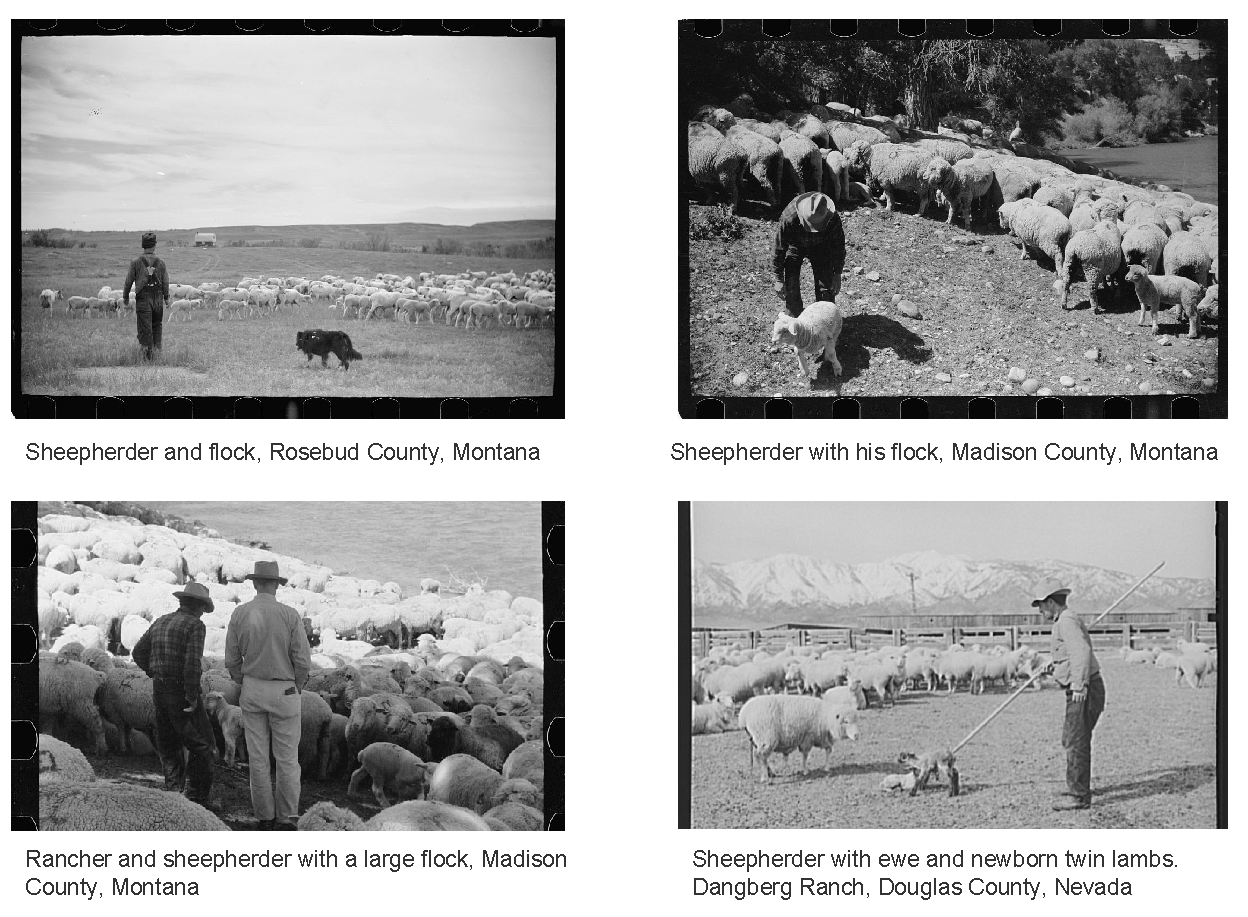
\includegraphics[width=0.45\textwidth]{introfigure.pdf}
\caption{ Here we show some sample images from the Historical Images Dataset that we are using in our work. Our objective is to generate these types of descriptions given these input images. The data is publicly available but we wrote a script to download both images, descriptions, and metadata.}
\label{fig:leadfigure}
\end{figure}

\section{Related Work}
Early work on image descriptions from photographs include~\cite{farhadi2010every,ordonez2011im2text} where image descriptions are retrieved using a nearest-neighbor approach based on some intermediate image representation. More recent works include the use of neural networks trained in an end-to-end fashion~\cite{showandtell,mao2014deep,karpathy2015deep}. Most of these previous work concentrate on image descriptions as a generic task, however we show in this work that a generic model doesn't translate well to specific domains such as the one presented in this report on historical images. To the best of our knowledge our work is one of the first to generate descriptions on historical images.

While there have been some previous work on historical images in multimedia~\cite{soo2002using,stvilia2010member}, most of the previous works have been for the task of image retrieval. We focus in our work instead on image descriptions which could also potentially help in the image retrieval task.

\begin{figure*}[t]
\centering
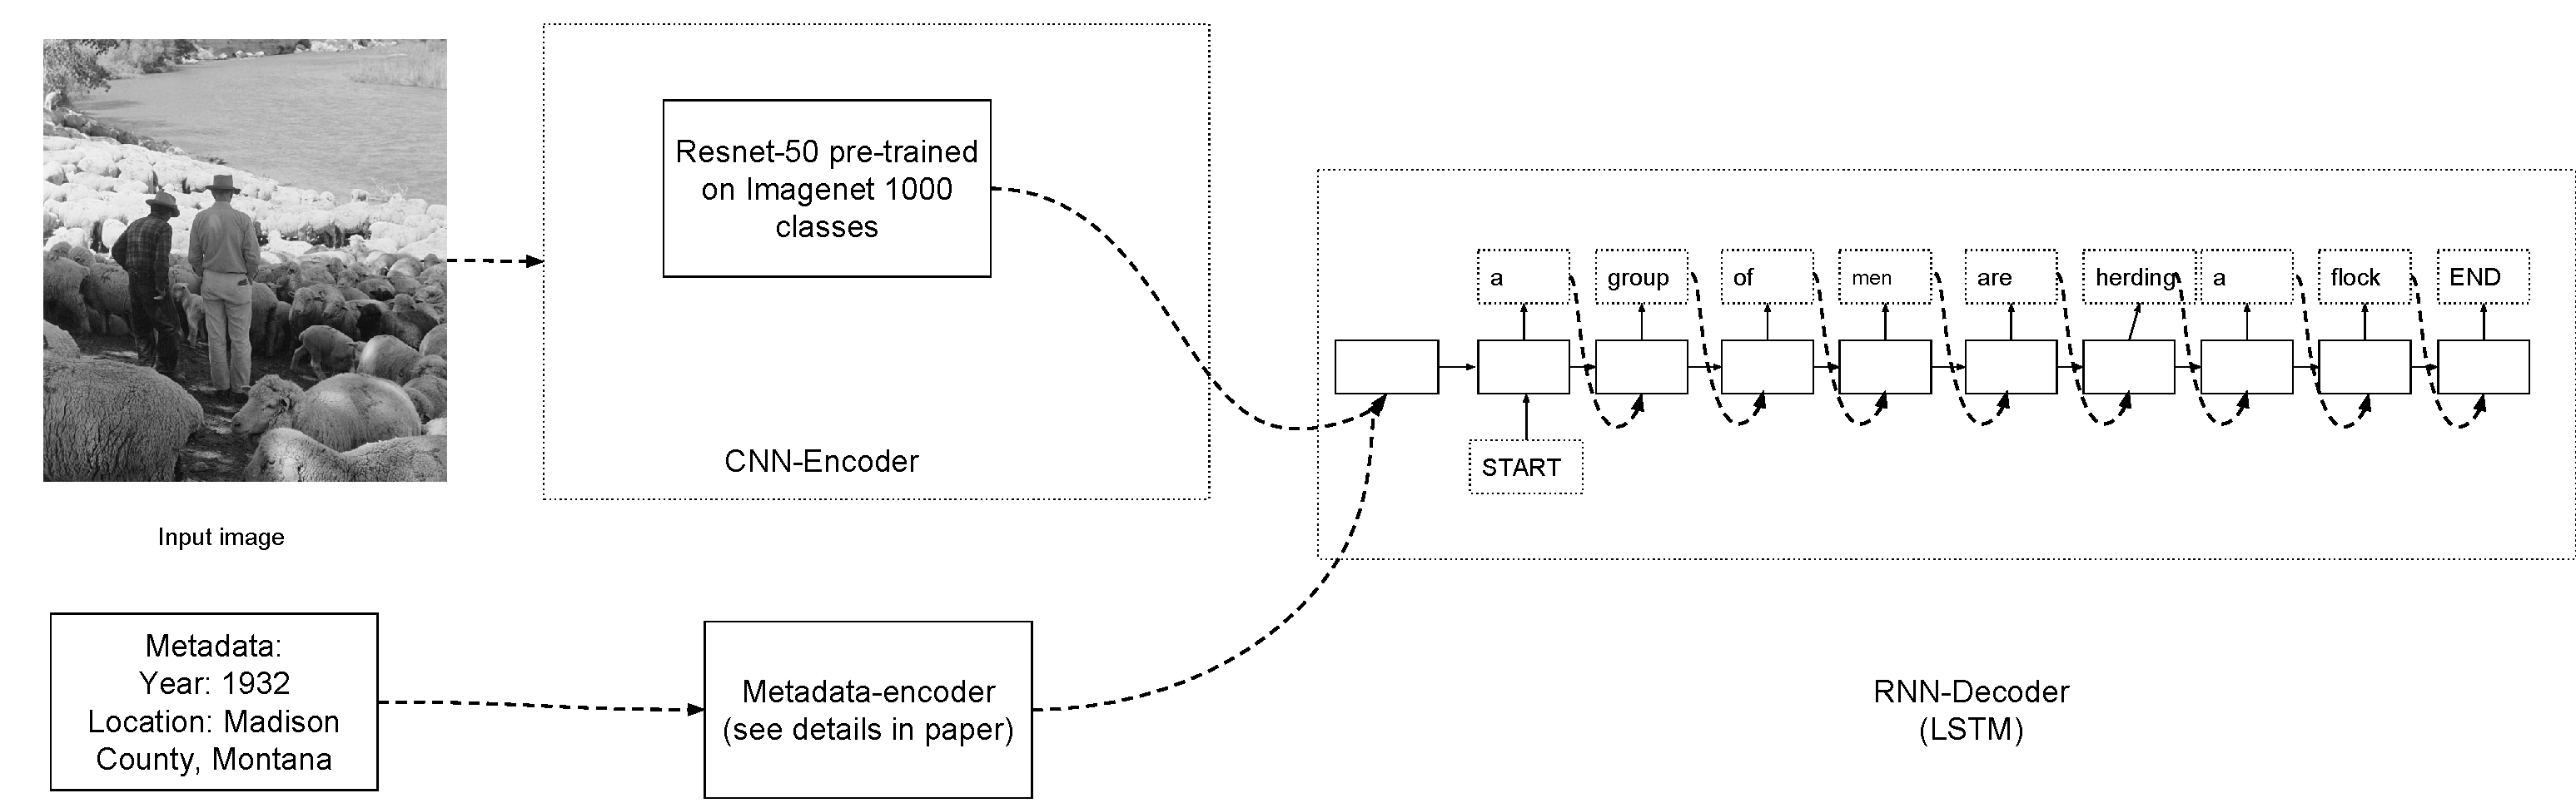
\includegraphics[width=0.9\textwidth]{overviewhistoric.pdf}
\caption{ Here we show a figure detailing our model components. The input is an image and a set of metadata. The output is a sequence of words.}
\label{fig:model}
\end{figure*}


\begin{table*}
\begin{center}
\begin{tabular}{ l  l  c  c  c }
\toprule
\textbf{Method} & \textbf{Train-data} & \textbf{BLEU} & \textbf{ROUGE} & \textbf{Perplexity} \\
\midrule
CNN+LSTM & MS-COCO &  [result]  & [result] & [result] \\
CNN+LSTM & HistoricImages & XX & XX & XX\\
CNN+LSTM+Context & HistoricImages + Year & XX & XX & XX\\
CNN+LSTM+Context & HistoricImages + Year + Location & XX & XX & XX\\
Gemma3-4B (Fine-Tuned) & HistoricImages + Year + Location & XX & XX & XX\\
\bottomrule
\end{tabular}
\end{center}
\caption{Preliminary experimental results comparing different models. XX marks pending results on planned experiments. The Gemma3 model is included as an additional baseline for evaluating the role of large-scale vision-language pretraining in historical image captioning.}
\label{table:results}
\end{table*}



%-------------------------------------------------------------------------
\section{Methodology}

We propose a modification of the standard encoder-decoder framework where the encoder consists of a pre-trained convolutional neural network (CNN), and thee decoder consists of a recurrent neural network (CNN). The modification consists on allowing another input to the language model consisting of metadata information from the input images (year, and location). A similar model was proposed by~\cite{yashimalearning} for e-commerce images that have additional categorical metadata. We show a schematic overview of our proposed model in Figure~\ref{fig:model}. Notice the extra inputs to the language model. In our experiments we used LSTMs for the recurrent networks.

In addition to our proposed CNN-RNN model, we also explore an alternative approach using a vision-language model (VLM) fine-tuned for historical image captioning. Specifically, we adapted the recently released Gemma-3 model~\footnote{\url{https://storage.googleapis.com/deepmind-media/gemma/Gemma3Report.pdf}}, which integrates a vision encoder with a transformer-based language decoder. The motivation behind using a VLM is to leverage its pre-trained knowledge, which includes multimodal information, while fine-tuning it to incorporate historical metadata for improved performance on domain-specific captioning.

The fine-tuning process involved training BLIP-2 on the historical images dataset with additional metadata embeddings injected into the transformer’s attention layers. This allows the model to learn contextual associations between the visual elements and the temporal and locational metadata. By leveraging pre-trained vision-language embeddings, the model can generate richer and more contextually appropriate captions compared to a CNN-RNN framework trained from scratch.

To evaluate the effectiveness of both approaches, we present a comparison of their performance using standard metrics in Table~\ref{table:results}.

\section{Experimental Settings}

\begin{figure}[b]
\centering
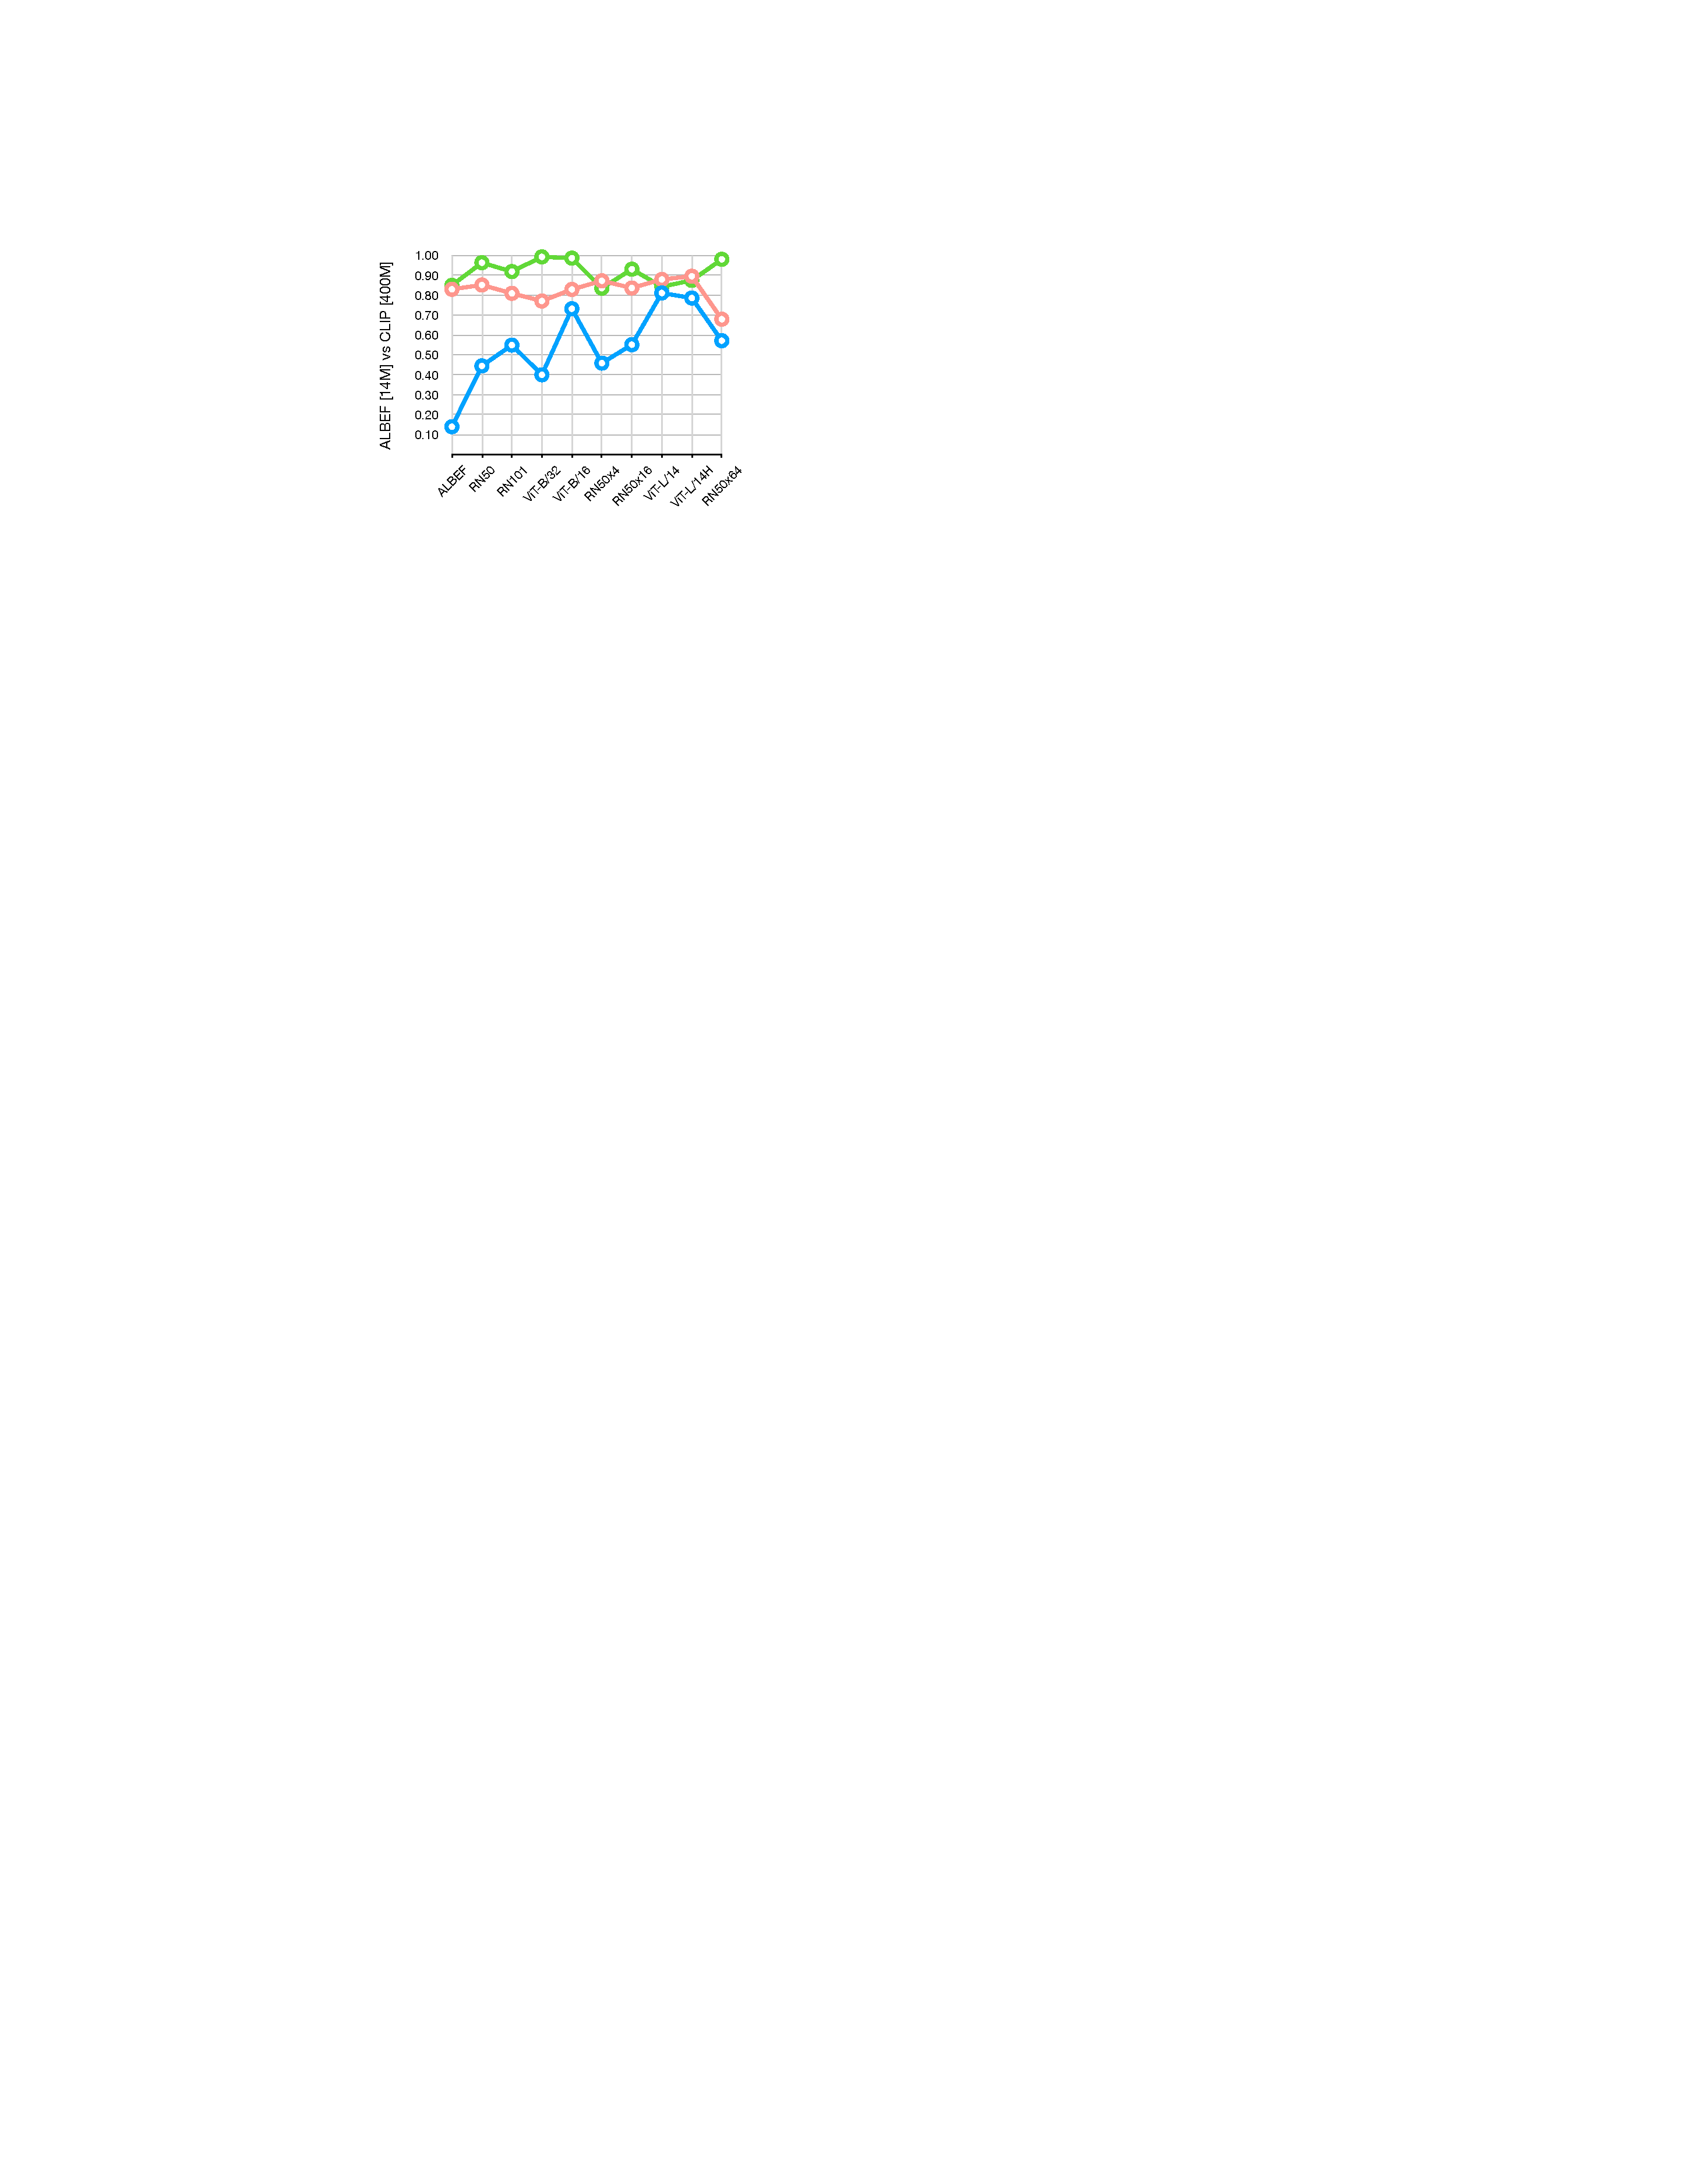
\includegraphics[width=0.48\textwidth]{dummy-figure.pdf}
\caption{This figure is also included only for illustrative purposes and does not reflect a real experiment. You should include actual results of your experiments. Notice that this figure is not an image, you can actually select the text on this figure. You can create your figures in matplotlib, powerpoint, etc but always has to be exported to PDF before being imported so text is selectable. Otherwise points deducted for presentation.}
\label{fig:loss}
\end{figure}

\begin{figure*}[th!]
\centering
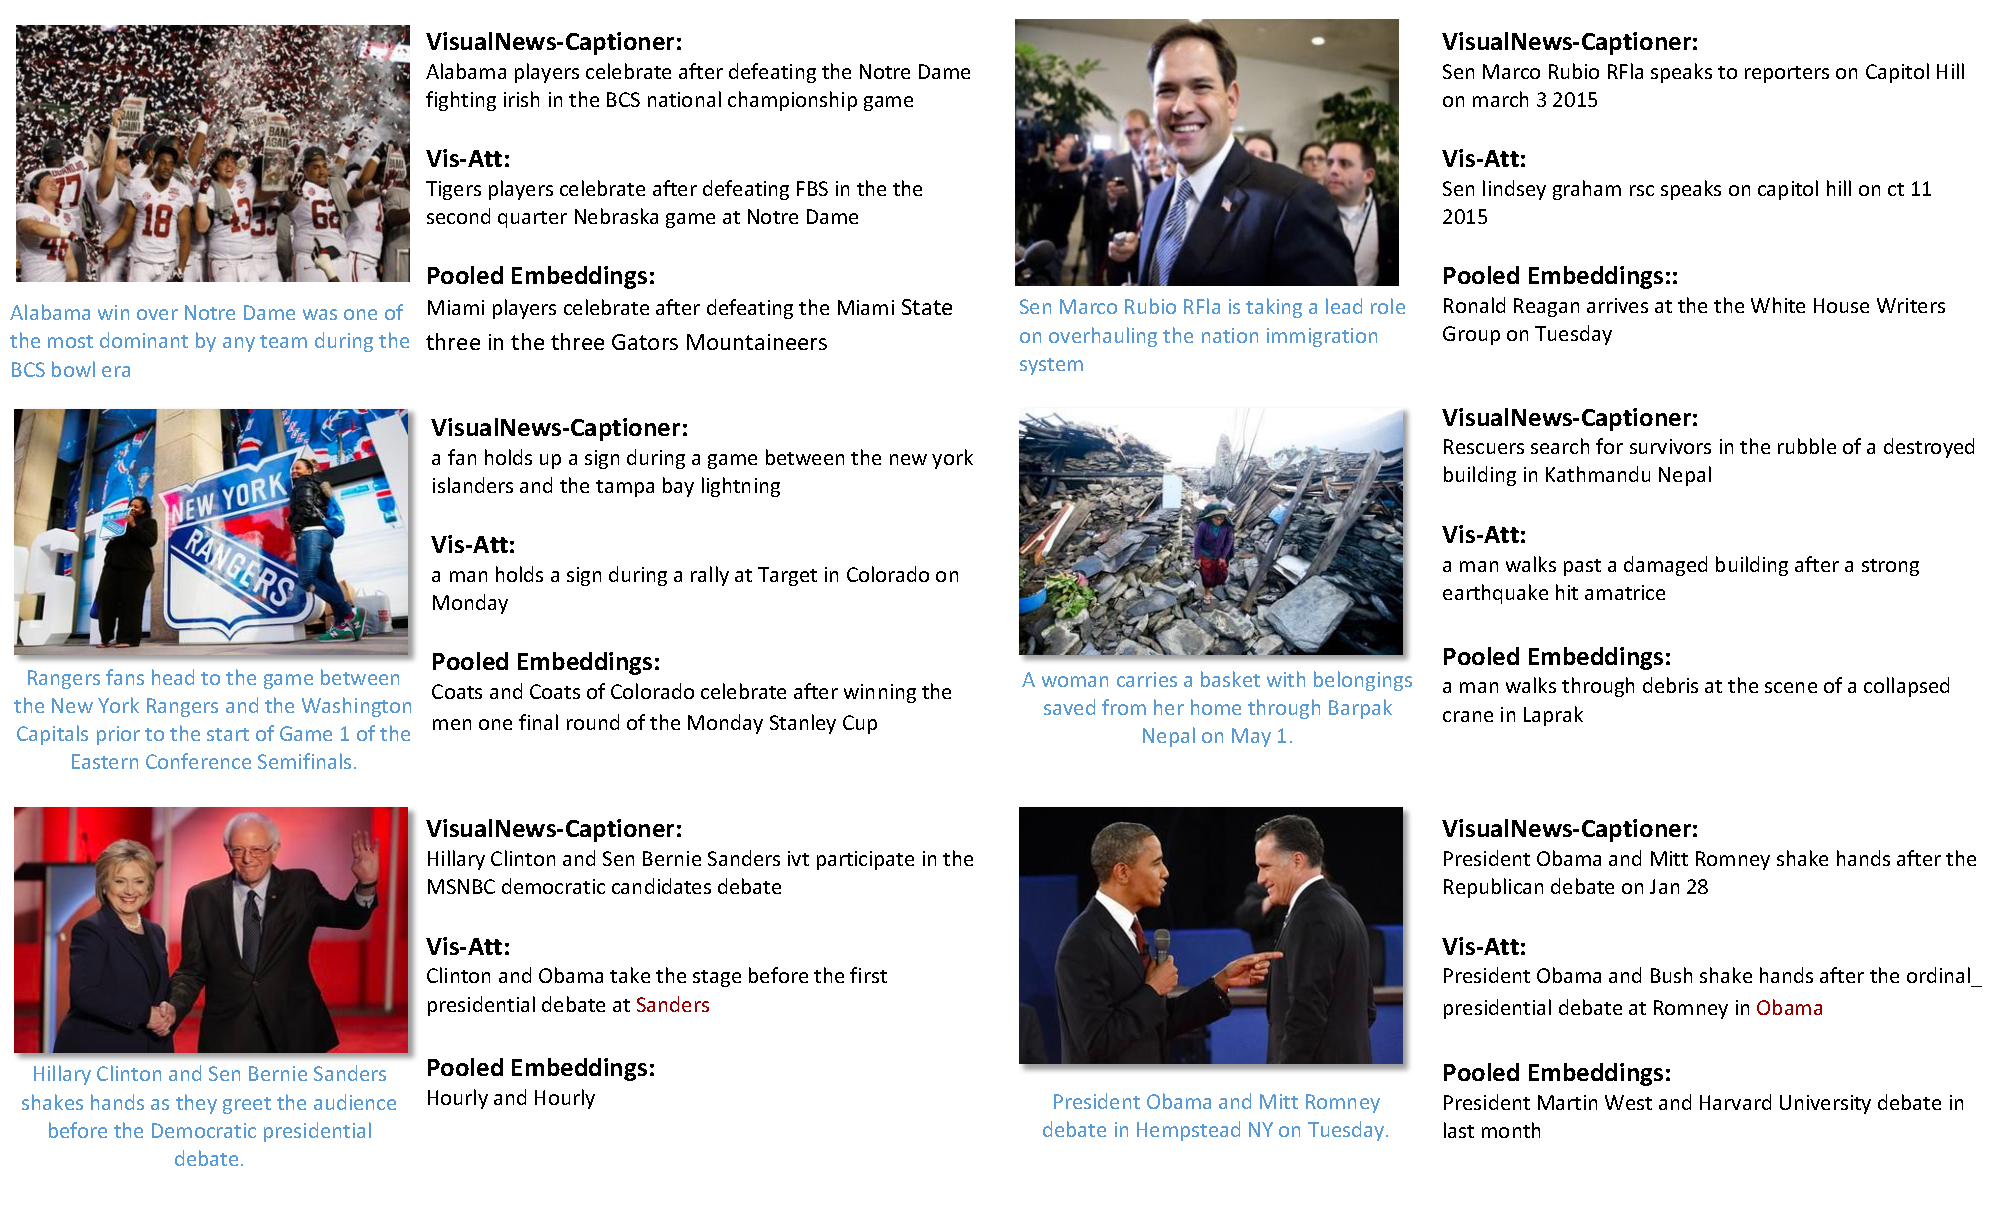
\includegraphics[width=\textwidth]{qualitative-news.pdf}
\caption{This figure is also included only for illustrative purposes and does not reflect a real experiment. You should include actual results of your experiments. Show some example results of your method. I generated this figure in powerpoint and then exported to PDF. Your figures should be at least of this quality. Properly exported into PDF before importing them with latex so that text is selectable. Points deducted otherwise for presentation.}
\label{fig:loss}
\end{figure*}

We used pytorch to implement our model, and used the code from a publicly available implementation as our starting implementation\footnote{\url{https://github.com/yunjey/pytorch-tutorial/tree/master/tutorials}}. We first trained the model on the standard MS-COCO dataset and run the model to predict captions directly on the HistoricImages dataset. We show the result of this experiment on the first row in Table~\ref{table:results}. We used the 50-layer version of the ResNet architecture~\cite{resnet} as our base deep convolutional network pre-trained in the ILSVRC task on Imagenet. We train our full model using stochastic gradient descent with momentum 0.9 and a mini-batch size of $64$. For all experiments, unless indicated otherwise, the learning rate was set to $1e-3$. The models were trained for a maximum of $60$ epochs. We show in Figure~\ref{fig:loss} the loss over time when we trained this baseline model. The images were isotropically scaled and cropped to a $256$x$256$ resolution and processed at a $224$x$224$ resolution by performing random crops and horizontal flips during training, and a center crop at test time. We still have not finished trained our model in the HistoricImages dataset but we have a working implementation. Additionally we have pending to implement the use of year and location as additional context but we have clear direction about how to do this.

In our final report we will additionally include sample outputs from our model showing side-by-side input images with metadata, and output captions obtained from our final model. Given our preliminary experiments we are confident that training on historical images should produce better results. 

\section{Analysis and Discussion}

In this section, we analyze the role of metadata in enhancing the quality of generated captions for historical photographs. Our experimental results indicate that integrating metadata, such as the year and location of an image, leads to significant improvements in caption accuracy, contextual relevance, and linguistic coherence. We discuss the key observations below.

\subsection{Impact of Metadata on Caption Accuracy}
One of the primary benefits of incorporating metadata is the improvement in caption accuracy. When trained solely on visual features, the model often generates generic descriptions that fail to capture the historical context of the images. However, when metadata such as the year and location is introduced, the model becomes more capable of producing descriptions that align with the historical period of the photograph. For instance, an image of a steam locomotive from the 1920s may initially be labeled simply as a "train," but with metadata, the caption can specify "A steam locomotive operating in the 1920s."

\subsection{Contextual Relevance and Historical Awareness}
Historical images often depict scenes, clothing, and technology that differ significantly from modern-day images. Without metadata, our model sometimes misclassifies historical elements, producing captions that use contemporary terminology inappropriate for the depicted time period. By providing metadata, the model has access to additional contextual cues that help refine descriptions. For example, a photograph from the 1940s depicting a wartime event is better understood when the model is informed that the image was captured during World War II.

\subsection{Reduction of Ambiguity in Caption Generation}
Metadata also plays a crucial role in reducing ambiguity in generated captions. Certain historical images contain objects or settings that could belong to multiple eras. Without contextual clues, the model may produce vague captions that lack specificity. For example, a photograph of a rural town may be described generically as "A town with buildings and streets," whereas with metadata, the caption could specify "A small rural town in the 1930s, with unpaved roads and vintage automobiles."

\subsection{Quantitative Performance Gains}
To quantitatively measure the impact of metadata, we compared model performance across several key evaluation metrics, including BLEU, ROUGE, and perplexity scores. Our results show a consistent improvement across all metrics when metadata is included. Table~\ref{table:results} presents the comparison of model performance with and without metadata. The increase in BLEU and ROUGE scores suggests that captions generated with metadata are more aligned with ground-truth descriptions.


\section{Conclusion}

In this project, we explored the task of generating automated descriptions for historical photographs using deep learning-based image captioning techniques. We built upon the standard encoder-decoder framework by incorporating additional metadata, such as the year and location of the image, to improve the relevance and contextual accuracy of the generated captions. Through our experiments, we demonstrated that training on domain-specific historical images, as opposed to general-purpose datasets like MS-COCO, significantly enhances the quality of the produced descriptions.

Our results indicate that models trained on historical image data are better equipped to capture the nuances of historical context, leading to more accurate and informative captions. Furthermore, the integration of metadata into the captioning process provides additional contextual cues that improve performance beyond visual features alone. This highlights the importance of multi-modal inputs for improving automatic caption generation in specialized domains.

Despite these promising results, there are several avenues for future work. One limitation of our approach is the reliance on existing metadata, which may not always be available or accurate. Future studies could explore methods for automatically inferring contextual information from visual cues alone. Additionally, leveraging more advanced natural language generation techniques, such as transformer-based models, could further enhance the fluency and coherence of the generated text. Finally, a user evaluation component could be introduced to assess the perceived quality of the captions in practical applications.

Overall, this work contributes to the growing field of automated historical image analysis by demonstrating the effectiveness of deep learning models for caption generation in a specialized domain. Our findings suggest that combining visual features with metadata can yield substantial improvements, paving the way for more robust and context-aware image captioning systems in the future.

\section{Ethical and Societal Considerations} The use of AI for historical image captioning raises ethical concerns, including bias, accuracy, and cultural sensitivity. AI models may inherit biases from historical data, leading to misleading or oversimplified descriptions, particularly for complex historical events. Ensuring accuracy requires expert-reviewed datasets, historical references, and human oversight. Sensitive images demand careful contextualization to avoid misrepresentation or trivialization of significant historical moments. While AI can improve access to historical archives, it should complement, not replace, expert interpretation. Future research should focus on explainable AI, interdisciplinary collaboration, and bias mitigation to ensure responsible and accurate historical AI applications.

\noindent
{\bf Acknowledgments. } We used Google Gemini Pro 2.0 to assist in editing and style. It was also helpful in suggesting a structure for the document but our ultimate report is our own responsibility and we stand by every word included in it. We also thank the authors of Mistral-7B which we use as our base model for the core of our experiments.





{\small
\bibliographystyle{ieee}
\bibliography{egbib}
}

\end{document}
